\subsection{Ay-Matak}
\label{sec:specie-ay-matak}

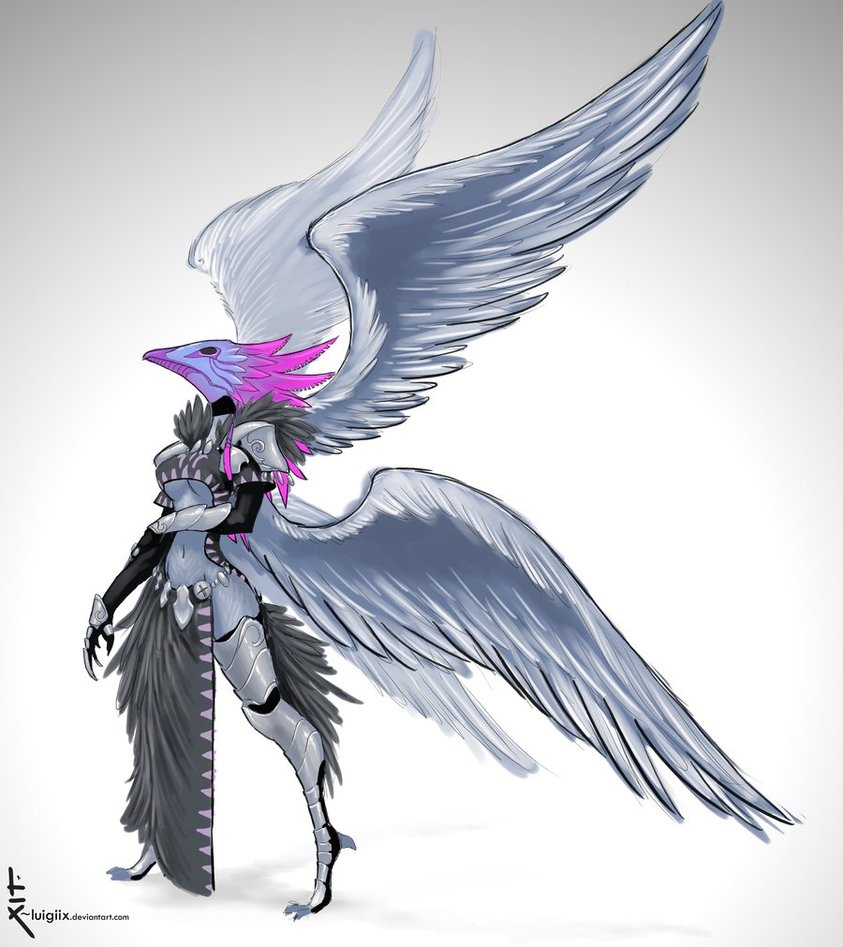
\includegraphics[width=\linewidth]{bird_race_f_concept_by_luigiix-d52w3as}

\begin{redtable}{\linewidth}{@{}L{.35}@{}L{.65}@{}}
  \textbf{Singular} & Matak\\
  \textbf{Plural} & Ay-Matak\\
  \textbf{Height} & 135-170cm\\
  \textbf{Weight} & 45-65kg\\
  \textbf{Gender Ratio} & 40\% Male / 60\% Female\\
  \textbf{Reproduction} & Oviparity (Eggs)\\
  \textbf{Maturity} & 15 years\\
  \textbf{Diet} & Omnivore\\
  \textbf{Homeworld} & Kitaba (Lost)
\end{redtable}

The Ay-Matak are an alien species that have evolved from the birds native to their homeworld of Kitaba. They are typically shorter and lighter than humans, have two pairs of wings, are bi-pedal, and have two arms with opposable thumbs on each of their hands. The beak is solid and sharp along the sides, with the tip made out of softer material that is flexible enough to produce a variety of sounds. The plumage of a male Matak is always more colourful than the female (who are limited to whites, greys and blacks).

Due to their wandering nature, many Ay-Matak were left stranded across the Black. The exact location of the homeworld has been lost, but what has been recovered from the databanks is that Kitaba was reknowned for its tall trees that almost touched the edges of the atmosphere. It also had a rich and diverse ecosystem that meant the Ay-Matak enjoyed an overabundance of food and had little need to compete for limited resources. Because of this the Ay-Matak were able to fully indulge in the pleasures of life. The Ay-Matak place a high social value on the arts (especially those that use an abundance of colour or visual stimuli), travel, and new ideas.

Planets with a majority of Ay-Matak are usually formed under an Oligarchic government. The members of the government are generally influential elders who have contributed greatly to the culture of the planet, or have travelled far and wide in search of new ideas.

To create a Matak character, please refer to the \textit{\hyperref[sec:rules-creation]{Character creation section}}

\textbf{Male Names:}

Andomion, Antakon, Artenaeon, Demoleo, Dralop, Entardion, Eraton, Eratro, Heliodo, Ikotu, Kalipon, Koron, Lokinu, Melaleimon, Myrodon, Panolio, Taramio, Teladon, Tridru, Tyrorion

\textbf{Female Names:}

Agara, Alanie, Aldorria, Anakia, Atria, Bellaleta, Belliana, Hallia, Iripira, Karellia, Katia, Kynie, Laleta, Nerian, Nolanta, Obemona, Peneleta, Talitian, Tiakia, Utriema

\textbf{Secondary Names:}

Ay-Matak do not take family names, but instead earn cultural "\textit{titles}" for their last well-known greatest achievement. For example, \textit{Andomion, painter of 'Matak Lost'}. Those without a great achievement usually go by their occupation, birthplace, spacecraft name, or include the name of their mother ("\textit{hatchling of Anakia}"). Needless to say that the Ay-Matak have caused headaches for many a bureacrat.
